% Figures. The sections call \FigureArch (text width, sec:intro), \FigureEncSeeds (column width, sec:encoder),
% \FigureLLM (text width, sec:llm) and \FigureExample (column width, sec:analysis).
% The two data-figure PDFs are drawn by clarity/paper_figures.py.

\newcommand{\FigureEncSeeds}{%
\begin{figure}[t]
\centering
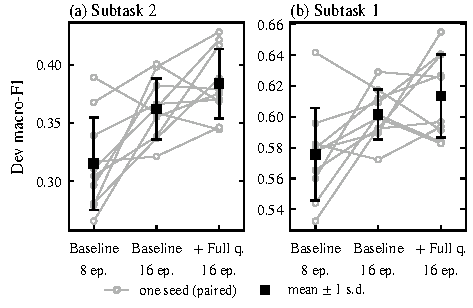
\includegraphics[width=\columnwidth]{figures/fig_deberta_seeds.pdf}
\caption{Single DeBERTa-v3-large models on dev for the three configurations: (a)~\Stwo{} multi-reference macro-F1, (b)~\Sone{} macro-F1. Open circles joined by thin lines are individual seeds, paired across configurations, and filled squares are the mean over the 10 seeds, with error bars of $\pm 1$ standard deviation.}
\label{fig:enc-seeds}
\end{figure}}

\newcommand{\FigureLLM}{%
\begin{figure*}[t]
\centering
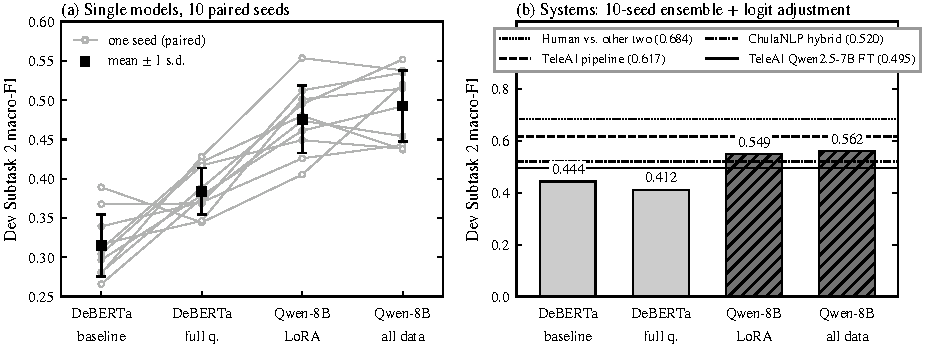
\includegraphics[width=\textwidth]{figures/fig_qwen_vs_deberta.pdf}
\caption{Dev \Stwo{} multi-reference macro-F1 of the DeBERTa-v3-large baseline, DeBERTa with the full question and 16 epochs, Qwen3-8B-Base with LoRA on the same input (3 epochs), and Qwen trained on all of train. (a)~Single models on 10 paired seeds: open circles joined by thin lines are individual seeds, and filled squares are means with $\pm 1$ standard deviation. (b)~The corresponding 10-seed systems (ensemble + logit adjustment, $\tau$ by nested CV, bar height the mean over 10 CV splits), with published dev results as horizontal lines: TeleAI's multi-call pipeline (0.617) and fine-tuned Qwen2.5-7B (0.495) \citep{shi-etal-2026-teleai}, ChulaNLP's DeBERTa top-5 + Kimi-K2 pipeline (0.52) \citep{peerachaidecho-rutherford-2026-chulanlp}, and a human annotator scored against the other two (0.684).}
\label{fig:llm}
\end{figure*}}

\newcommand{\FigureArch}{%
\begin{figure*}[t]
\centering
% Figure 1: the classification pipeline (TikZ, monochrome). Input by \FigureArch in figs.tex.
\begin{tikzpicture}[
  font=\small,
  node distance=2.6mm,
  box/.style={draw, rounded corners=1.5pt, align=center, inner xsep=3pt, inner ysep=3pt, minimum height=#1},
  box/.default=19mm,
  sub/.style={draw, rounded corners=1.5pt, align=center, inner sep=2.5pt, minimum width=#1},
  sub/.default=25mm,
  arr/.style={-{Stealth[length=4pt]}, thin},
  note/.style={font=\footnotesize\itshape, align=center},
  band/.style={draw, densely dotted, rounded corners=2pt, inner sep=2.5pt, align=center, font=\footnotesize},
]
% Input
\node[box, fill=black!6] (in) {%
  \textbf{Input}\\[2pt]
  sub-question $q$\\
  full question $Q$\\
  answer $a$\\[1pt]
  {\footnotesize $\le$ 1{,}024 tokens}};

% Backbone: one of two
\node[sub, right=of in, yshift=5.2mm] (deb) {\textbf{DeBERTa-v3-large}\\{\footnotesize fine-tuned, \texttt{[CLS]}}};
\node[sub, right=of in, yshift=-5.2mm] (qwen) {\textbf{Qwen3-8B-Base}\\{\footnotesize LoRA, last token}};
\node[draw, dashed, rounded corners=2pt, inner sep=2pt, fit=(deb)(qwen)] (bb) {};
\node[note, above=0.3mm of bb] {backbone (one of)};

% Head
\node[box, right=of bb] (head) {\textbf{Linear head}\\[2pt] 9 logits\\ softmax\\[1pt] $p_s(c \mid x)$};

% Seed ensemble: stacked outlines stand for the ten trained seeds
\node[box, right=of head, fill=white] (ens) {\textbf{Mean over}\\\textbf{10 seeds}\\[3pt] $\bar p(c \mid x)$};
\begin{scope}[on background layer]
  \draw[rounded corners=1.5pt, fill=white] ($(ens.south west)+(1.2mm,1.2mm)$) rectangle ($(ens.north east)+(1.2mm,1.2mm)$);
  \draw[rounded corners=1.5pt, fill=white] ($(ens.south west)+(0.6mm,0.6mm)$) rectangle ($(ens.north east)+(0.6mm,0.6mm)$);
\end{scope}

% Logit adjustment
\node[box, right=of ens, xshift=1.2mm] (la) {\textbf{Logit adjustment}\\[2pt]
  $\arg\max\limits_c \dfrac{\bar p(c \mid x)}{\pi_c^{\,\tau}}$};

% Outputs
\node[sub=20mm, fill=black!6, right=of la, yshift=6.6mm] (s2) {\textbf{Subtask 2}\\{\footnotesize evasion type (9)}};
\node[sub=20mm, fill=black!6, right=of la, yshift=-6.6mm] (s1) {\textbf{Subtask 1}\\{\footnotesize clarity level (3)}};

% Arrows
\draw[arr] (in) -- (bb);
\draw[arr] (bb) -- (head);
\draw[arr] (head) -- (ens);
\draw[arr] ($(ens.east)+(1.2mm,0)$) -- (la);
\draw[arr] (la.east) -- ++(1.8mm,0) |- (s2.west);
\draw[arr] (s2) -- (s1);

% Training and decision notes
\path let \p1=(in.west), \p2=(head.east), \p3=(bb.south) in
  node[band, anchor=north, text width=\x2-\x1-5pt] at ({(\x1+\x2)/2}, \y3-2mm) (train) {%
  \textit{Training, per seed:} 3{,}103 train rows, cross-entropy, epoch chosen on the 345-row train slice};
\path let \p1=(ens.west), \p2=(s1.east), \p3=(train.north) in
  node[band, anchor=north, text width=\x2-\x1-5pt] at ({(\x1+\x2)/2}, \y3) (dec) {%
  \textit{Decision:} $\pi_c$ is the class prior on train, and $\tau$ (nested CV) is the only parameter fitted on dev};
\end{tikzpicture}

\caption{The classification system. One backbone (DeBERTa-v3-large, fully fine-tuned, or Qwen3-8B-Base with LoRA) reads the sub-question, the journalist's full question and the answer, and a new linear head gives a distribution over the nine evasion types. A system averages ten seeds and applies logit adjustment, which divides by the train class prior $\pi_c$ raised to $\tau$. The Subtask~1 clarity level follows from the Subtask~2 label through the fixed taxonomy.}
\label{fig:arch}
\end{figure*}}

\newcommand{\FigureExample}{%
\begin{figure}[t]
\centering
\small
\begin{tabular}{@{}p{0.97\columnwidth}@{}}
\toprule
\textbf{Sub-question:} Would you campaign against Senator Joe Lieberman on Iraq? \\
\textbf{Full question:} \ldots{} would you campaign against Senator Joe Lieberman, whose Republican candidate may support you, but he supports you too, on Iraq? \\
\textbf{Answer:} I'm going to stay out of Connecticut. \\
\textbf{Annotators:} Dodging, Dodging, Implicit (\Sone{}: Ambivalent) \\
\bottomrule
\end{tabular}

\medskip
\setlength{\tabcolsep}{4pt}
\begin{tabular}{@{}lll@{}}
\toprule
 & DeBERTa system & Qwen system \\
\midrule
$\bar p$, top 3 & General .373 & Dodging .327 \\
                & Implicit .282 & Implicit .189 \\
                & Deflection .205 & Declining .170 \\
Ensemble argmax & General $\times$ & Dodging $\checkmark$ \\
$\tau$ (item's fold) & 0.70 & 0.85 \\
\Stwo{} after LA & General $\times$ & Declining $\times$ \\
\Sone{} & Ambivalent $\checkmark$ & Clear Non-Reply $\times$ \\
\bottomrule
\end{tabular}
\caption{One dev item through both 10-seed systems ($\checkmark$: in the reference set, or for \Sone{} the gold level). The item was fixed in advance as the error discussed in \S\ref{sec:analysis}. Qwen ranks an acceptable label first, but logit adjustment divides by the train prior (0.205 for Dodging, 0.042 for Declining to answer) and moves the decision to the rarer class.}
\label{fig:example}
\end{figure}}

\newcommand{\FigurePlan}{%
\begin{figure*}[t]
\centering
% Planned system for the final evaluation (TikZ, monochrome, same style as fig_architecture.tex).
% Input by \FigurePlan in figs.tex. Everything in this figure is planned, not run.
% Row 1: input -> M1 -> M2 -> output.  Row 2: M4 (left, under M1) and M3 (right, under M2).
\begin{tikzpicture}[
  font=\footnotesize,
  box/.style={draw, rounded corners=1.5pt, align=center, inner xsep=3pt, inner ysep=3pt},
  plan/.style={box, dashed},
  arr/.style={-{Stealth[length=4pt]}, thin},
  lab/.style={font=\footnotesize, inner sep=1.5pt},
]
% Row 1
\node[box, fill=black!6] (in) {\textbf{Input}\\[1pt] $q$, $Q$, $a$};
\node[plan, right=3.5mm of in] (m1) {\textbf{M1}\enspace Candidate generator\\[1pt]
  {\footnotesize Qwen3-8B + LoRA, $K$ seeds, logit adjustment}\\[1pt]
  {\footnotesize $\bar p(c \mid x)$, candidate set $C(x)$, uncertainty $u(x)$}};
\node[plan, right=5mm of m1] (m2) {\textbf{M2}\enspace Router\\[1pt]
  {\footnotesize defer the fraction $\delta$}\\{\footnotesize with the highest $u(x)$}};
\node[box, fill=black!6, right=18mm of m2] (out) {\textbf{Subtask 2}\\[1pt]{\footnotesize $\rightarrow$ Subtask 1}};

% Row 2
\node[plan, anchor=north west, text width=74mm] (m3) at ($(in.west |- m2.south)+(45mm,-6mm)$) {%
  \centering\textbf{M3}\enspace LLM adjudicator\\[1pt]
  {\footnotesize an open-weight LLM scores only the labels in $C(x)$,
  given definitions, a confusion guide and boundary examples
  retrieved from similar training items, fused with $\bar p$,
  then logit adjustment}};
\node[plan, anchor=north west, text width=36mm] (m4) at (in.west |- m3.north) {%
  \centering\textbf{M4}\enspace Distillation\\[1pt]
  {\footnotesize the adjudicator's decisions on train become
  soft targets for M1, 4-bit inference}};

% Arrows
\draw[arr] (in) -- (m1);
\draw[arr] (m1) -- (m2);
\draw[arr] (m2) -- node[lab, above] {keep, $1-\delta$} (out);
\draw[arr] (m2.south) -- node[lab, right] {defer, $\delta$} (m2.south |- m3.north);
\draw[arr] (m3.east) -| (out.south);
\draw[arr, densely dashed] (m3.west |- m4.east) -- (m4.east);
\draw[arr, densely dashed] (m4.north -| m1.south west) ++(6mm,0) -- ($(m1.south west)+(6mm,0)$);
\end{tikzpicture}

\caption{The planned system for the final evaluation (dashed boxes are new modules, none run yet, see \S\ref{sec:conclusion}). LLM calls per item equal $\delta$, against 1.94 for the winning system \citep{shi-etal-2026-teleai}.}
\label{fig:plan}
\end{figure*}}
